%
%Не забыть:
%--------------------------------------
%Вставить колонтитулы, поменять название на титульнике



%--------------------------------------

\documentclass[a4paper, 12pt]{article} 

%--------------------------------------
%Russian-specific packages
%--------------------------------------
%\usepackage[warn]{mathtext}
\usepackage[T2A]{fontenc}
\usepackage[utf8]{inputenc}
\usepackage[english,russian]{babel}
\usepackage[intlimits]{amsmath}
\usepackage{esint}
%--------------------------------------
%Hyphenation rules
%--------------------------------------
\usepackage{hyphenat}
\hyphenation{ма-те-ма-ти-ка вос-ста-нав-ли-вать}
%--------------------------------------
%Packages
%--------------------------------------
\usepackage{amsmath}
\usepackage{amssymb}
\usepackage{amsfonts}
\usepackage{amsthm}
\usepackage{latexsym}
\usepackage{mathtools}
\usepackage{etoolbox}%Булевые операторы
\usepackage{extsizes}%Выставление произвольного шрифта в \documentclass
\usepackage{geometry}%Разметка листа
\usepackage{indentfirst}
\usepackage{wrapfig}%Создание обтекаемых текстом объектов
\usepackage{fancyhdr}%Создание колонтитулов
\usepackage{setspace}%Настройка интерлиньяжа
\usepackage{lastpage}%Вывод номера последней страницы в документе, \lastpage
\usepackage{soul}%Изменение параметров начертания
\usepackage{hyperref}%Две строчки с настройкой гиперссылок внутри получаеммого
\usepackage[usenames,dvipsnames,svgnames,table,rgb]{xcolor}% pdf-документа
\usepackage{multicol}%Позволяет писать текст в несколько колонок
\usepackage{cite}%Работа с библиографией
\usepackage{subfigure}% Человеческая вставка нескольких картинок
\usepackage{tikz}%Рисование рисунков
\usepackage{float}% Возможность ставить H в положениях картинки
% Для картинок Моти
\usepackage{misccorr}
\usepackage{lscape}
\usepackage{cmap}





\usepackage{graphicx,xcolor}
\graphicspath{{Pictures/}}
\DeclareGraphicsExtensions{.pdf,.png,.jpg}

%----------------------------------------
%Список окружений
%----------------------------------------
\newenvironment {theor}[2]
{\smallskip \par \textbf{#1.} \textit{#2}  \par $\blacktriangleleft$}
{\flushright{$\blacktriangleright$} \medskip \par} %лемма/теорема с доказательством
\newenvironment {proofn}
{\par $\blacktriangleleft$}
{$\blacktriangleright$ \par} %доказательство
%----------------------------------------
%Список команд
%----------------------------------------
\newcommand{\grad}
{\mathop{\mathrm{grad}}\nolimits\,} %градиент

\newcommand{\diver}
{\mathop{\mathrm{div}}\nolimits\,} %дивергенция

\newcommand{\rot}
{\ensuremath{\mathrm{rot}}\,}

\newcommand{\Def}[1]
{\underline{\textbf{#1}}} %определение

\newcommand{\RN}[1]
{\MakeUppercase{\romannumeral #1}} %римские цифры

\newcommand {\theornp}[2]
{\textbf{#1.} \textit{ #2} \par} %Написание леммы/теоремы без доказательства

\newcommand{\qrq}
{\ensuremath{\quad \Rightarrow \quad}} %Человеческий знак следствия

\newcommand{\qlrq}
{\ensuremath{\quad \Leftrightarrow \quad}} %Человеческий знак равносильности

\renewcommand{\phi}{\varphi} %Нормальный знак фи

\newcommand{\me}
{\ensuremath{\mathbb{E}}}

\newcommand{\md}
{\ensuremath{\mathbb{D}}}



%\renewcommand{\vec}{\overline}




%----------------------------------------
%Разметка листа
%----------------------------------------
\geometry{top = 3cm}
\geometry{bottom = 2cm}
\geometry{left = 1.5cm}
\geometry{right = 1.5cm}
%----------------------------------------
%Колонтитулы
%----------------------------------------
\pagestyle{fancy}%Создание колонтитулов
\fancyhead{}
%\fancyfoot{}
%----------------------------------------
%Интерлиньяж (расстояния между строчками)
%----------------------------------------
%\onehalfspacing -- интерлиньяж 1.5
%\doublespacing -- интерлиньяж 2
%----------------------------------------
%Настройка гиперссылок
%----------------------------------------
\hypersetup{				% Гиперссылки
	unicode=true,           % русские буквы в раздела PDF
	pdftitle={Заголовок},   % Заголовок
	pdfauthor={Автор},      % Автор
	pdfsubject={Тема},      % Тема
	pdfcreator={Создатель}, % Создатель
	pdfproducer={Производитель}, % Производитель
	pdfkeywords={keyword1} {key2} {key3}, % Ключевые слова
	colorlinks=true,       	% false: ссылки в рамках; true: цветные ссылки
	linkcolor=blue,          % внутренние ссылки
	citecolor=blue,        % на библиографию
	filecolor=magenta,      % на файлы
	urlcolor=cyan           % на URL
}
%----------------------------------------
%Работа с библиографией (как бич)
%----------------------------------------
\renewcommand{\refname}{Список литературы}%Изменение названия списка литературы для article
%\renewcommand{\bibname}{Список литературы}%Изменение названия списка литературы для book и report
%----------------------------------------
\begin{document}
	\begin{titlepage}
		\begin{center}
			$$$$
			$$$$
			$$$$
			$$$$
			{\Large{НАЦИОНАЛЬНЫЙ ИССЛЕДОВАТЕЛЬСКИЙ УНИВЕРСИТЕТ}}\\
			\vspace{0.1cm}
			{\Large{ВЫСШАЯ ШКОЛА ЭКОНОМИКИ}}\\
			\vspace{0.25cm}
			{\large{Факультет физики}}\\
			\vspace{5.5cm}
			{\Huge\textbf{{Лабораторная работа}}}\\%Общее название
			\vspace{1cm}
			{Работу выполнили студенты 3 курса}\\
			{Захаров Сергей Дмитриевич}\\
			{и Исаков Александр Валерьевич}
			\vfill
			
\includegraphics[width = 0.2\textwidth]{HSElogo}\\
			\vfill
			Москва\\
			2021
		\end{center}
	\end{titlepage}
	
	\tableofcontents
	
	\newpage
	
	\section{Постановка цели}
	
	
	
	\subsection{Оже-спектроскопия}
	
	В роли исследуемого образца выступает некое сыпучее вещество, спеченное или спрессованное в форму цилиндрической таблетки. Необходимо внести ее в вакуумную камеру после предварительной подготовки, затем получить получить Оже-спектр, после чего путем его анализа определить, из каких элементов состоит образец.
	
	\subsection{Сканирующая туннельная микроскопия}
	
	В этой части в роли исследуемого образца выступает уже внесенный в вакуум графит. На нем необходимо получить обзорный СТМ-кадр, по которому нужно определить высоту ступеньки. 
	
	Затем необходимо получить СТМ-изображение с атомным разрешением и определить межатомное расстояние. После этого, путем изменения напряжения, при котором производится сканирование, определить, как при этом меняется профиль изображения.
	
	%Кроме того, на исследуемом образце также присутствует т.н. муаровый узор, возникший при наложении нескольких слоев решетки графита, повернутых друг относительно друга на некоторый угол. С помощью моделирования необходимо определить взаимное расположение слоев, дающих присутствующий рисунок.
	
	\section{Оже-спектроскопия}
	
	\subsection{Принцип метода}
	
	Мы пользуемся тем фактом, что энергия связи электронов глубоких оболочек атома чувствительна к природе элемента, что позволяет, измеряя кинетическую энергию эмитированных с поверхности под действием фотонной или электронной бомбардировки, получать информацию об \textbf{элементном} составе поверхности. Мы также пользуемся тем, что электроны с кинетической энергией 15-1000~эВ обладают очень маленькими длинами свободного пробега в веществе, что позволяет получать информацию только о поверхности, не затрагивая толщу образца.
	
	При бомбардировке образца электронами с энергией порядка 3000~эВ происходит несколько параллельных процессов. Во-первых, упругое рассеяние электронов на электронных оболочках атомов. Эти электроны покидают образец без изменения энергии. Во-вторых, неупругое рассеяние электронов на электронных оболочках атомов, в частности нас интересует рассеяние на электронах внутренних оболочек атомов.
	
	Мы рассматриваем т.н. оже-пики, которые появляются вследствие т.н. оже-процесса. Схема процесса представлена на рисунке \ref{fig:1_diag} и состоит из трех этапов. Сперва первичный электрон с энергией порядка 2-3~кЭв выбивает электрон с оболочки атома (этот электрон называется вторичным), образуя тем самым вакансию (а). После этого происходит релаксация за счет внутреннего перехода электрона с более высокого уровня на получившуюся вакансию (б). Наконец, испускается оже-электрон, который мы детектируем и кинетическую энергию которого мы измеряем (в).
	
	\begin{figure}[H]
		\centering
		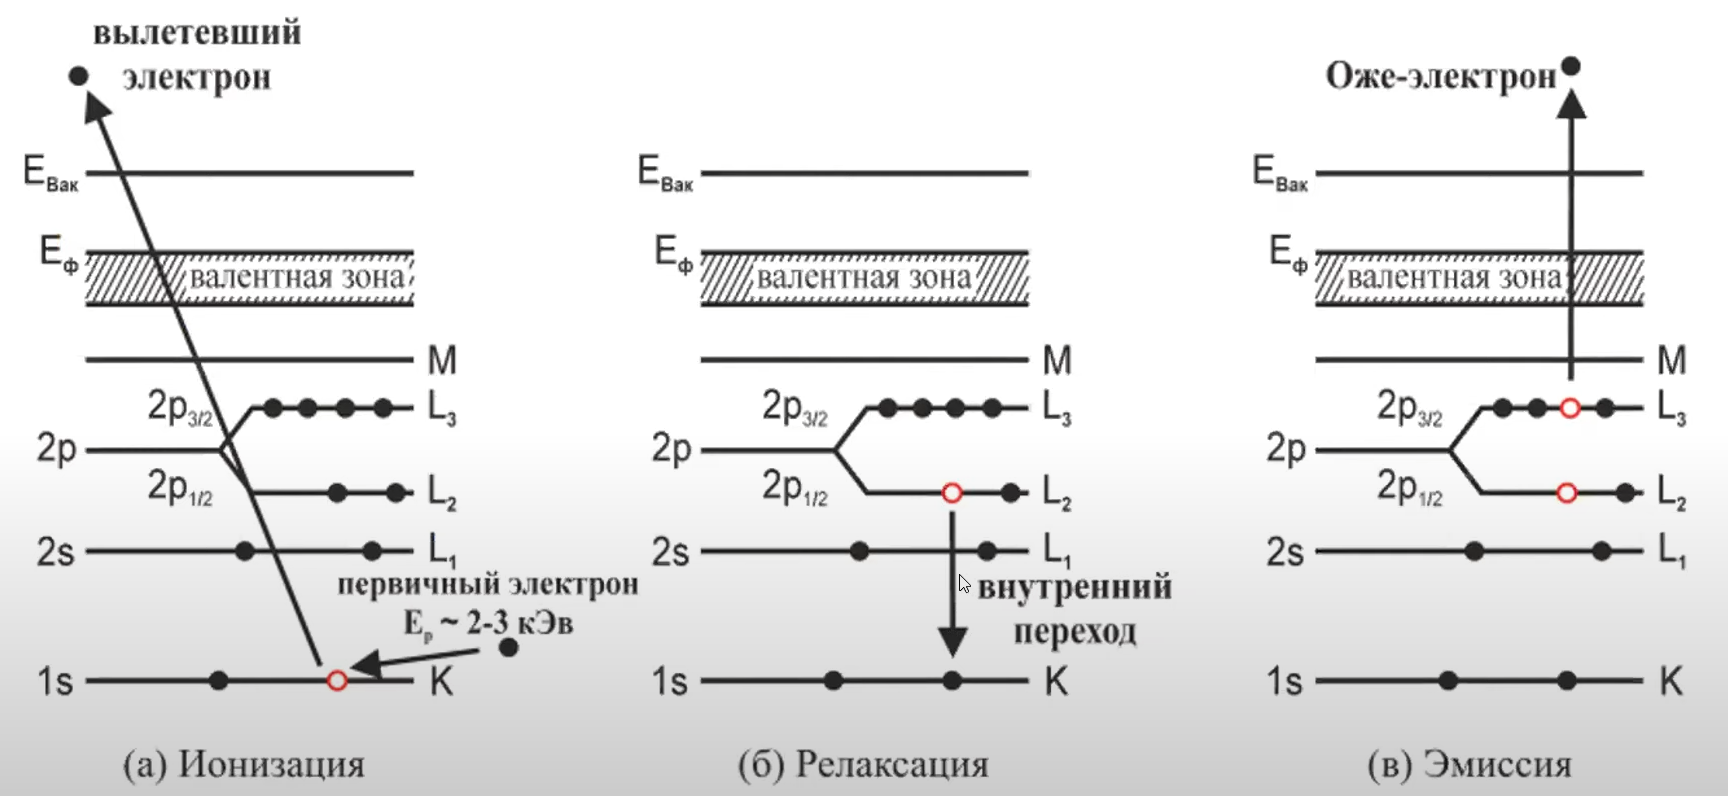
\includegraphics[width=0.7\linewidth]{1_diag}
		\caption{Схематическая иллюстрация оже-процесса из \cite{Auge_diag}.}
		\label{fig:1_diag}
	\end{figure}
	
	\subsection{Подготовка образца для внесения в вакуум}
	
	Первоначально предлагалось закрепить образец на держателе с помощью танталовой нити с использованием контактной сварки, однако спустя несколько неудачных попыток было решено, что данный способ при отсутствии должной практики затруднителен в практическом исполнении, принимая во внимание факт, что образец имеет цилиндрической формы. По этой причине было решено <<накрыть>> образец танталовой пластиной, предварительно просверлив в ней отверстие достаточного диаметра для получения Оже-спектра и сделав <<ножки>>, с помощью которых образец бы держался между пластинами.
	
	%\begin{figure}[H]
	%	\centering
	%	\includegraphics[width=0.7\linewidth]{1_fastening}
	%	\caption{Крепление образца с помощью танталовой пластины.}
	%	\label{fig:1_fastening}
	%\end{figure}
	
	\subsection{Анализ оже-спектра}
	
	Изначально был получен оже-спектр при бомбардировке образца электронами с энергией 3000~эВ с помощью установки, описанной в \cite{Auger_spectr}. С учетом возможности наличия т.н. пиков потерь, которые находятся в той же области, что и оже-пики, было решено проверить их присутствие за счет увеличения энергии бомбардирующих электронов на 500~эВ. В таком случае оже-пики, которые являются характеристикой вещества, должны были бы остаться на месте, а пики потерь --- сместиться. Из рисунка \ref{fig:1_Auge_double} видно, что смещения ни одного из пиков не наблюдается, что свидетельствует о том, что все пики являются оже-пиками.
	
	\begin{figure}[H]
		\centering
		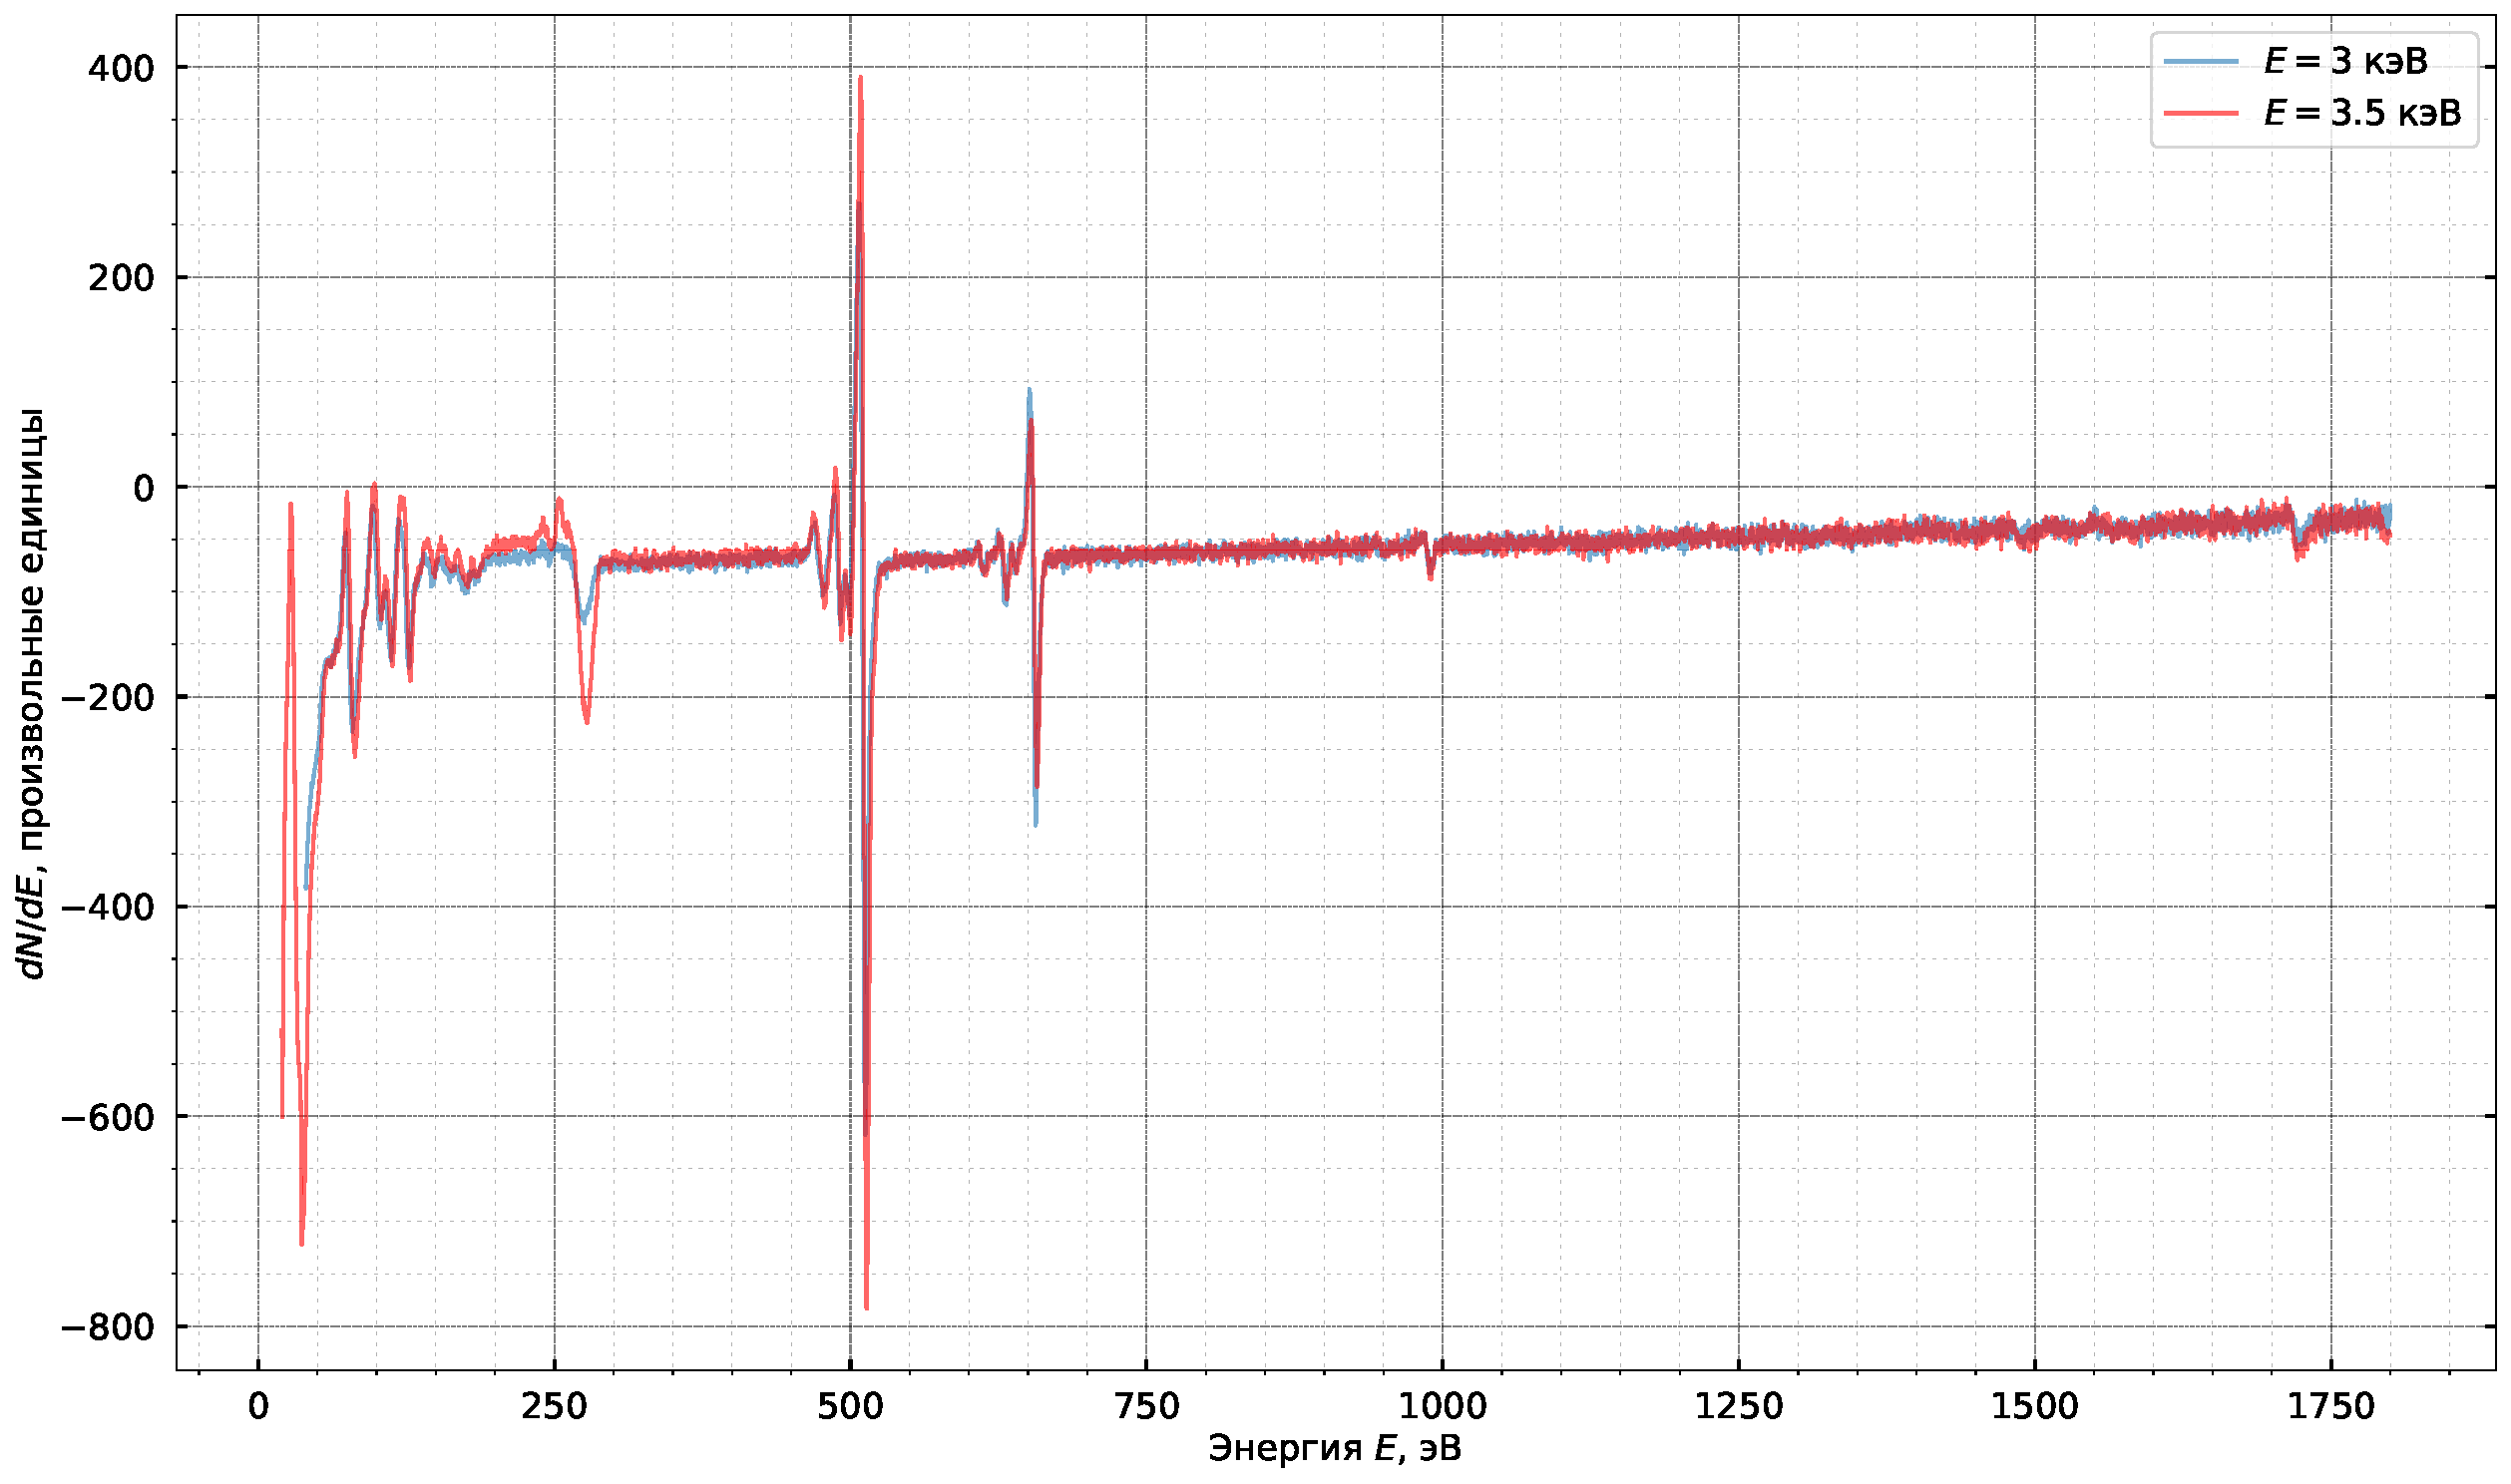
\includegraphics[width=0.9\linewidth]{1_Auge_double}
		\caption{Сравнение Оже-спектров, полученных при 3000~эВ и 3500~эВ.}
		\label{fig:1_Auge_double}
	\end{figure}

	После того, как стало ясно, что все пики являются оже-пиками, можно приступить к анализу полученных спектров. Каталожными обычно являются спектры, снятые при 3000~эВ и 5000~эВ. Из-за ограничений, накладываемых на нас имеющейся установкой, мы можем получить только спектры 3000~эВ и 3500~эВ, поскольку б\`{о}льшая энергия электронов на недоступна. Тем не менее, даже спектра 3500~эВ оказалось достаточно, чтобы внести некоторую ясность в структуру полученных данных. Проанализированный спектр 3000~эВ представлен на рисунке \ref{fig:1_Auge_3000}.
	
	Как было сказано, спектр 3500~эВ оказался полезен в <<дальней>> части спектра: с его помощью был выявлено наличие еще одного пика, предположительно, тулия. Кроме того, благодаря тому, что это сканирование мы запустили с меньшего нижнего порога по энергиям, на нем также виден пик натрия в самом начале спектра. Расшифрованный оже-спектр представлен на рисунке \ref{fig:1_Auge_3500}. 
	
	В качестве каталожных спектров были взяты спектры из \cite{Auger}.
	
	\begin{figure}[H]
		\centering
		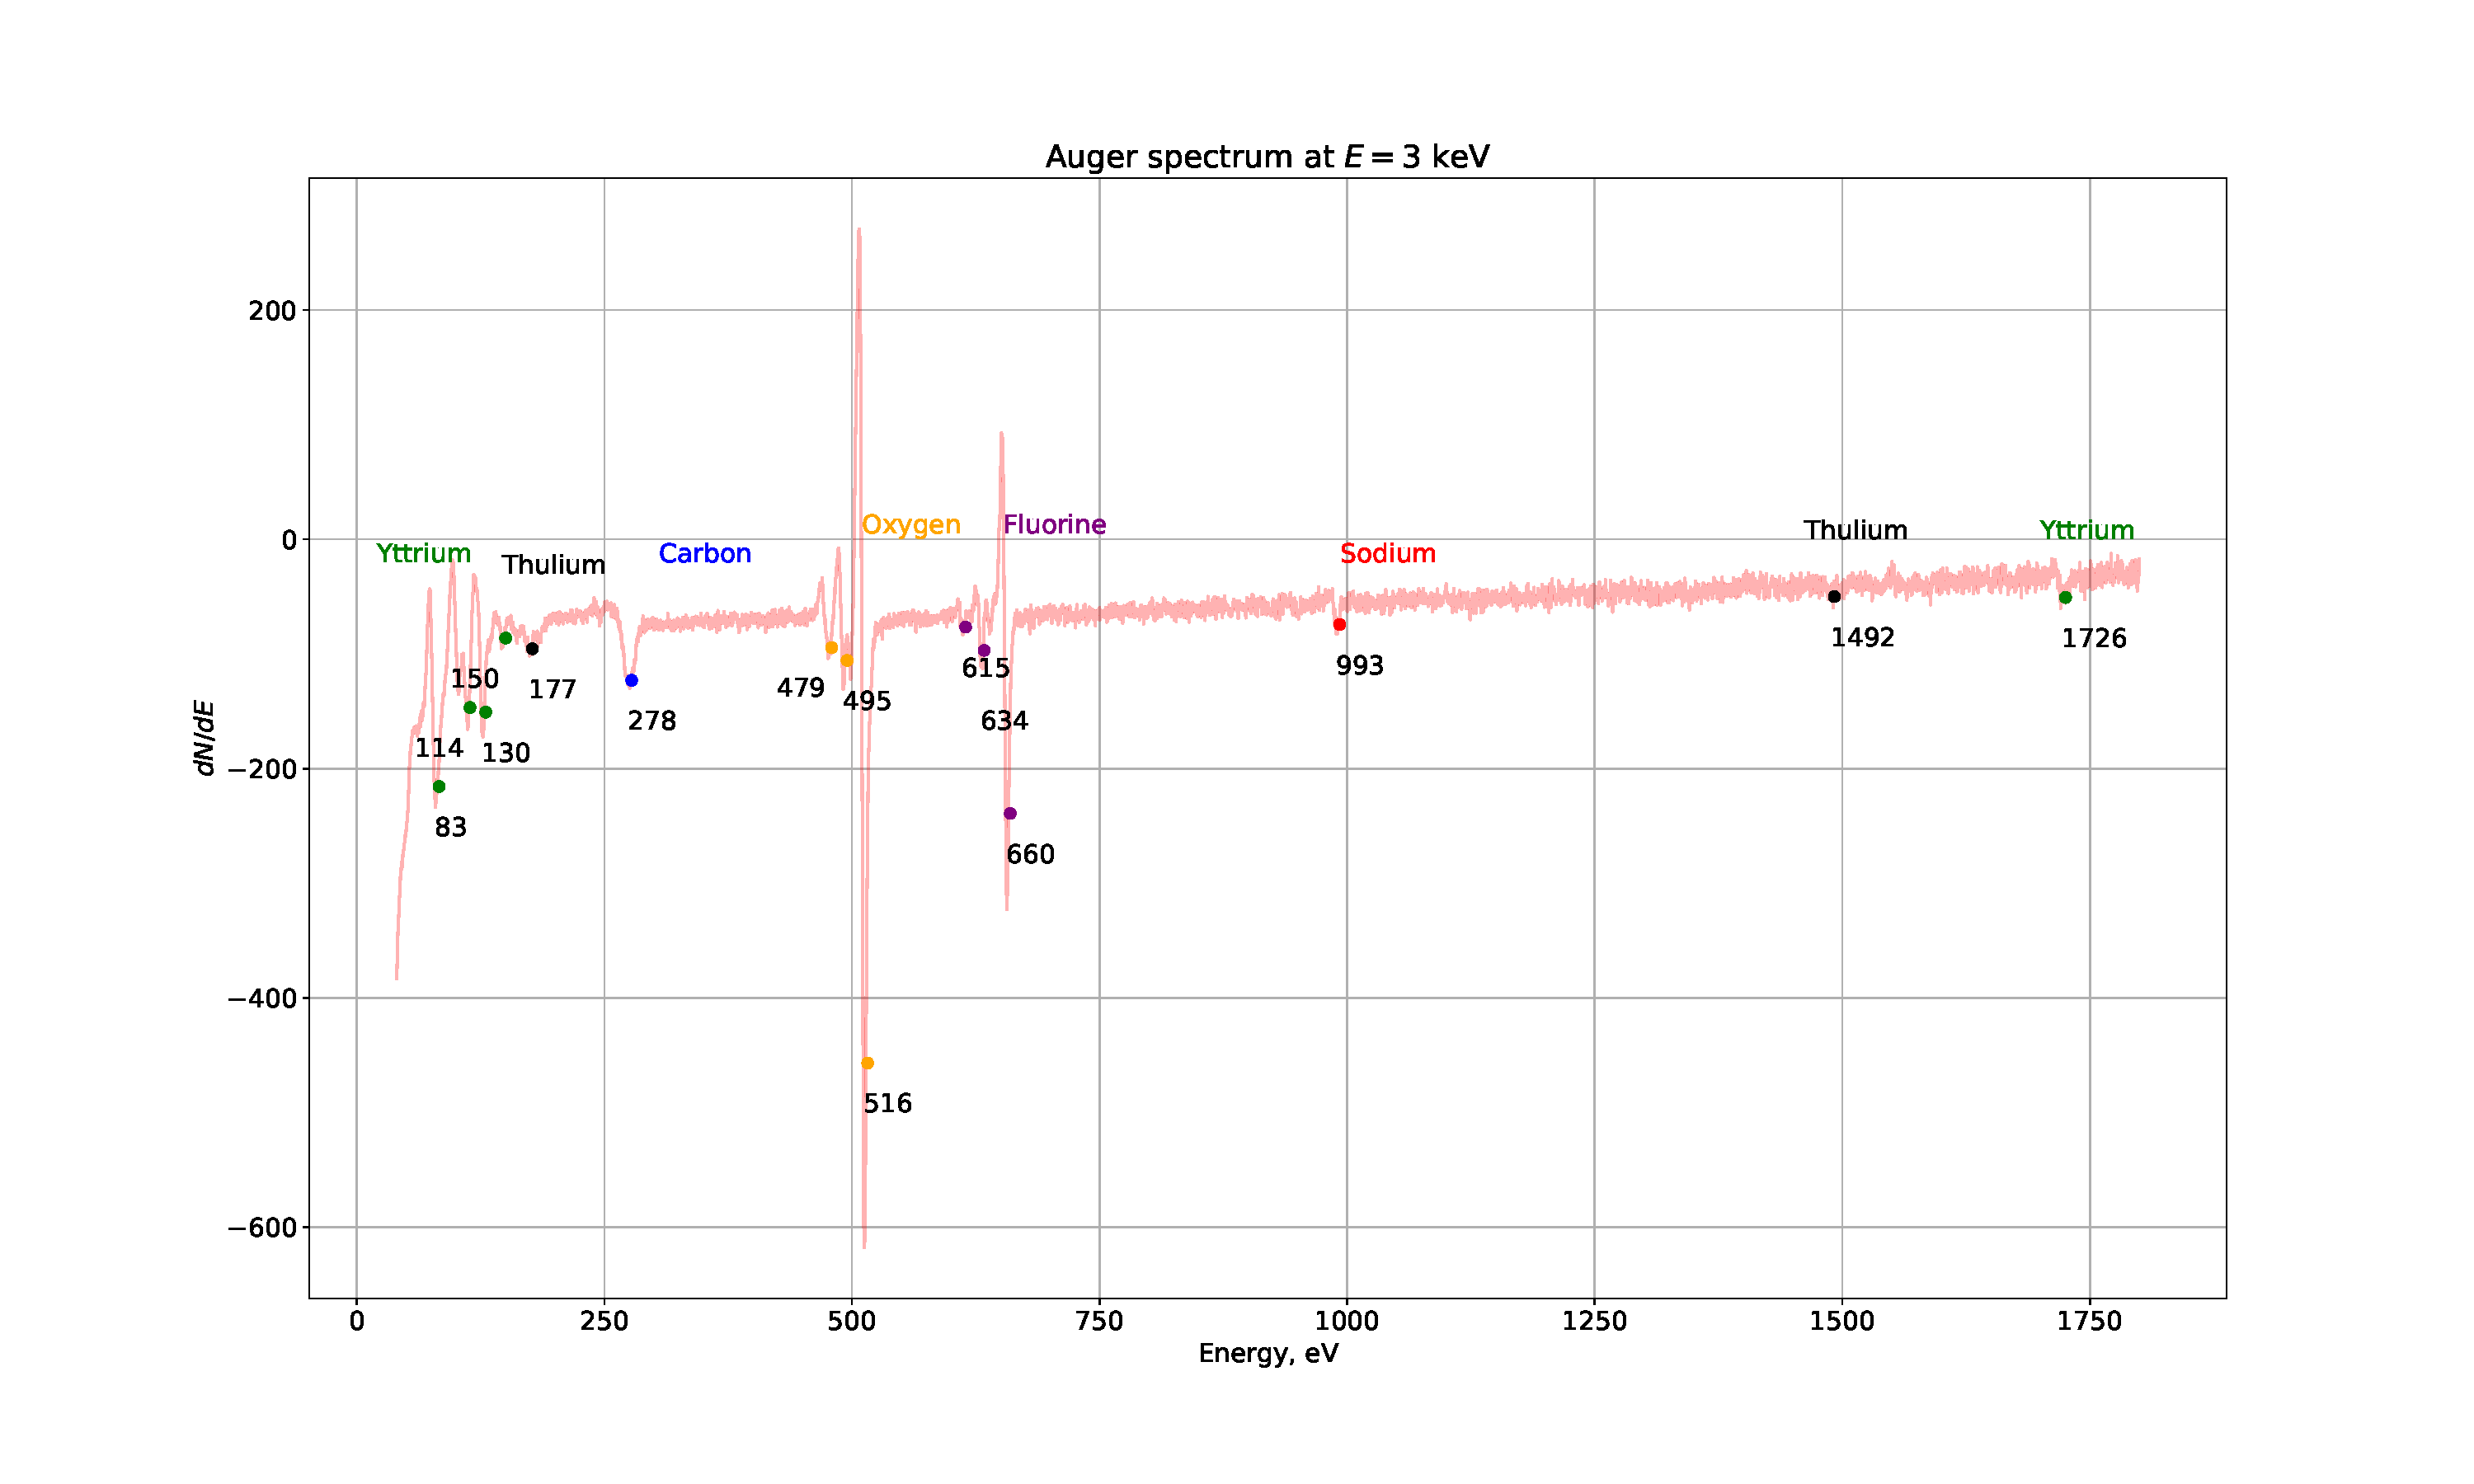
\includegraphics[width=0.9\linewidth]{1_Auge_3000}
		\caption{Полученный Оже-спектр 3000~эВ с нанесенными названиями элементов, дающих пики.}
		\label{fig:1_Auge_3000}
	\end{figure}
	
	\begin{figure}[H]
		\centering
		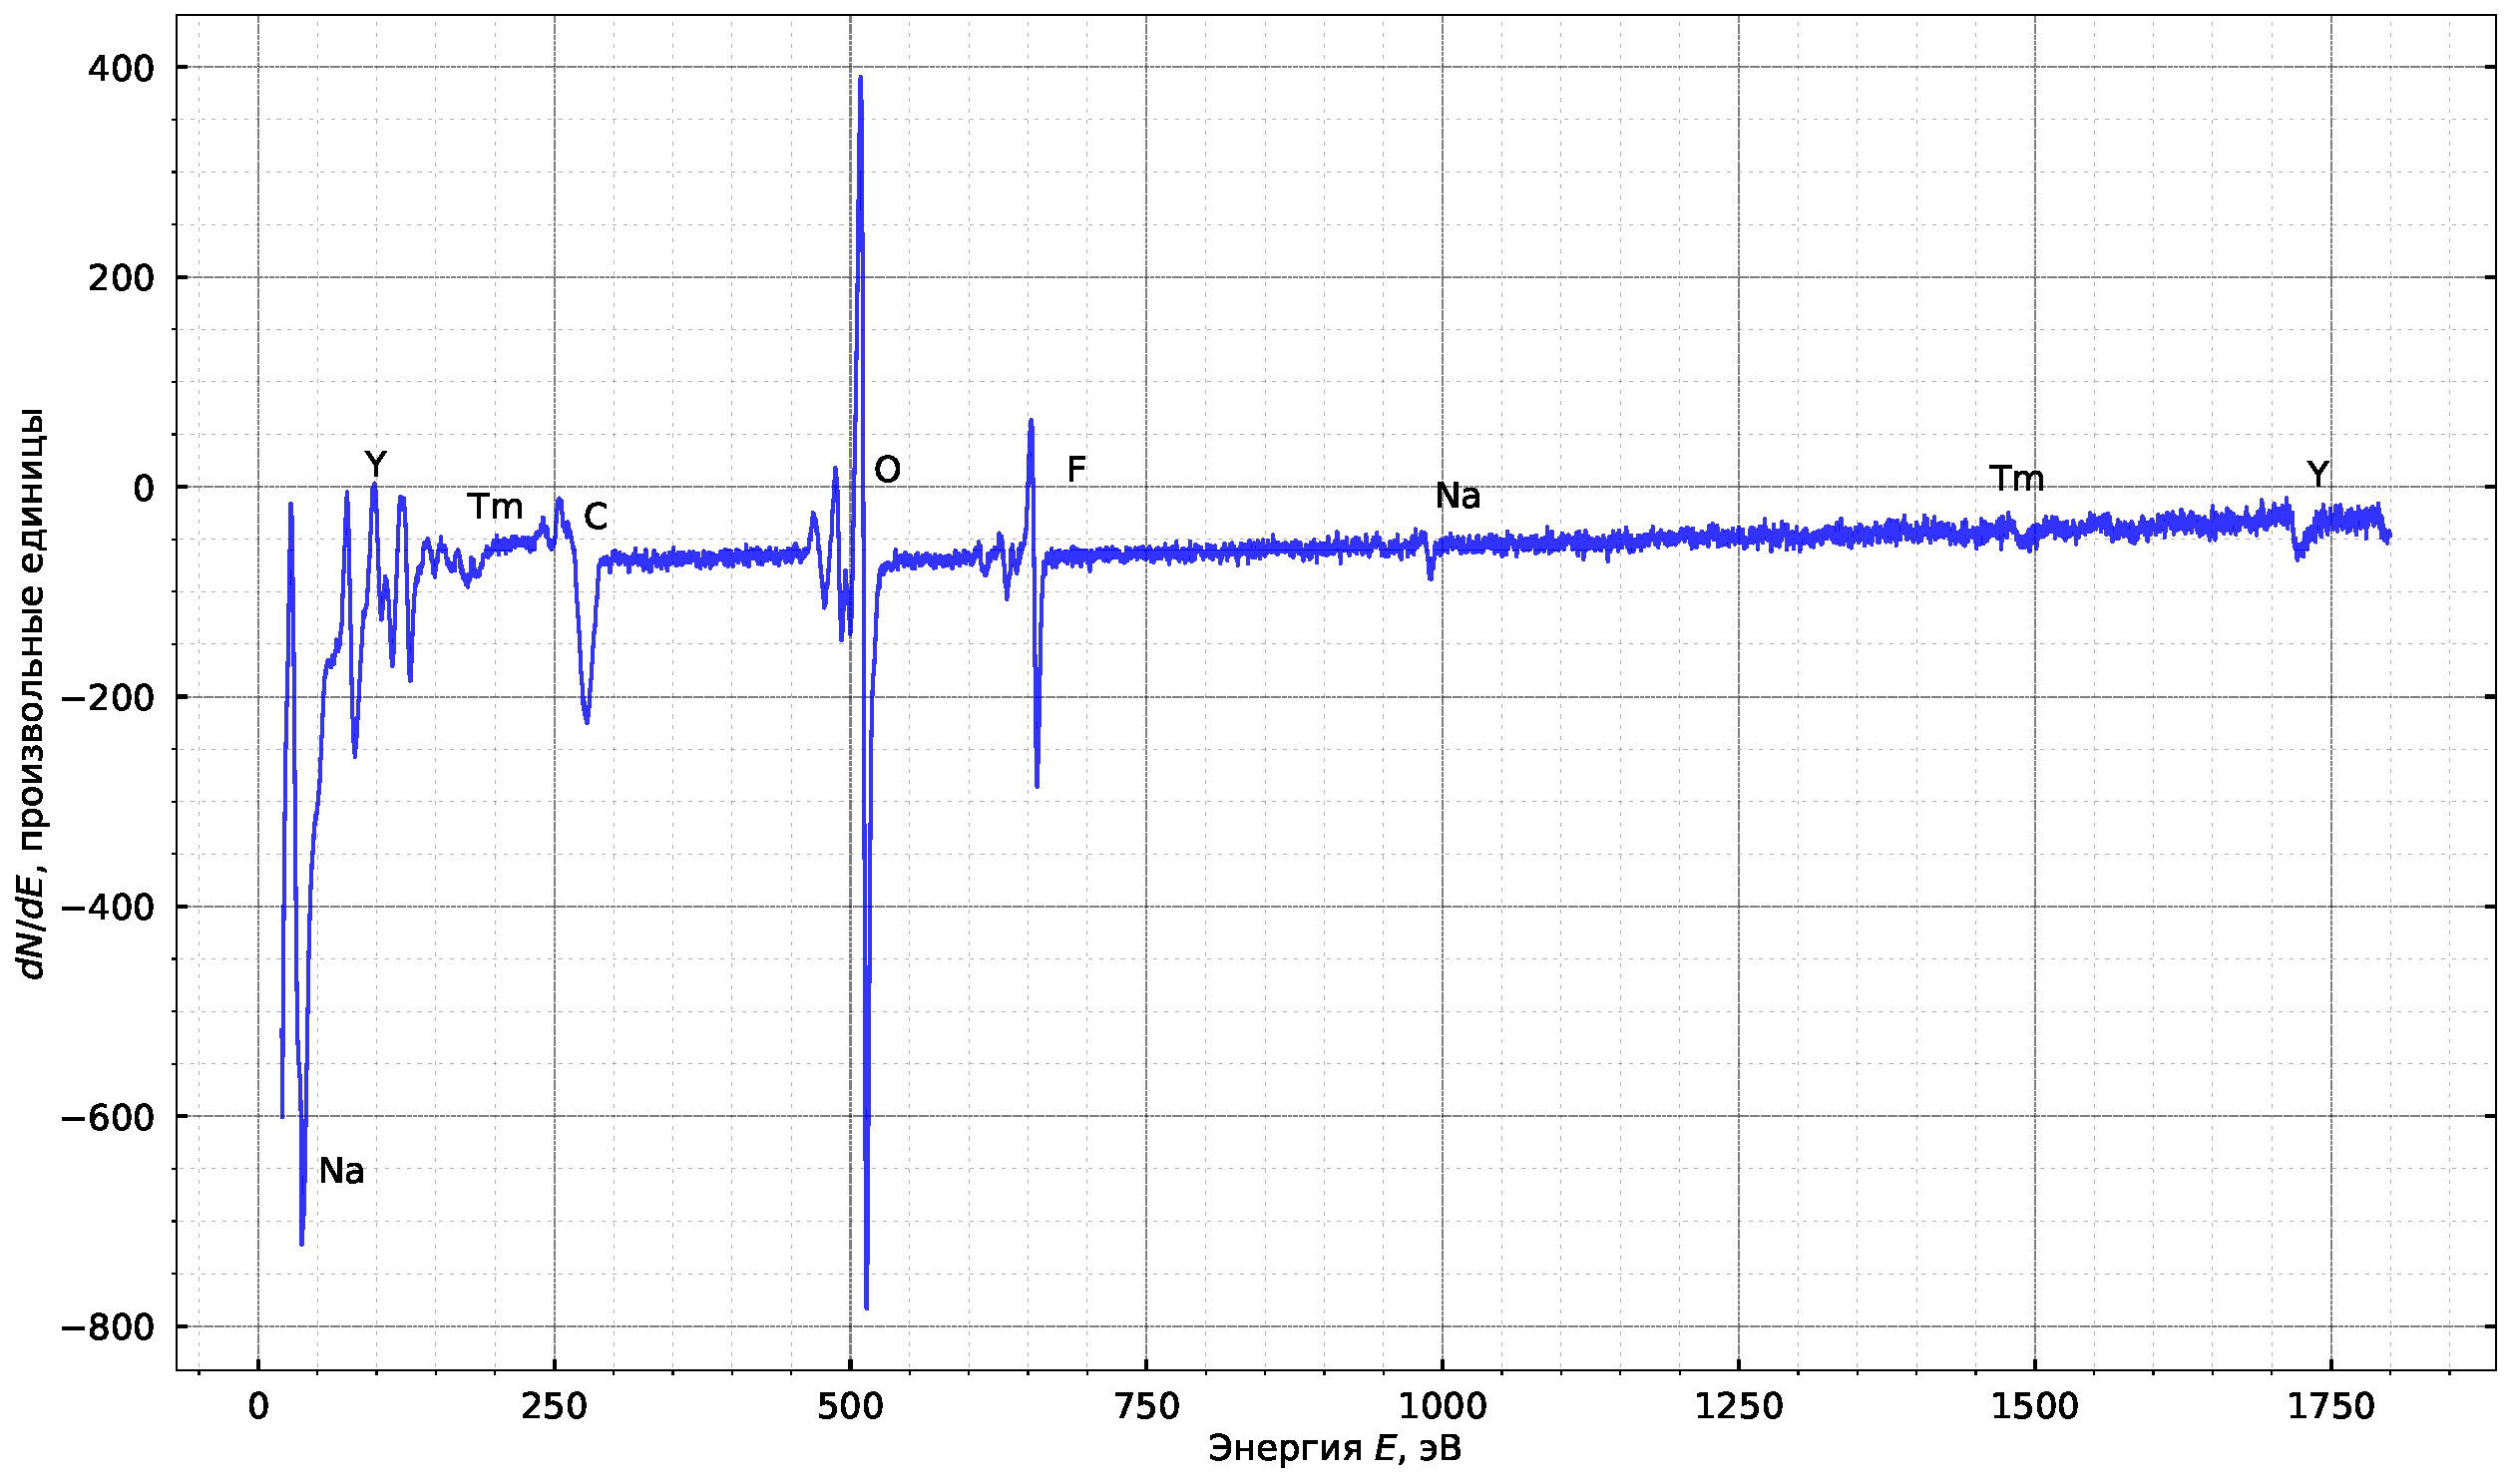
\includegraphics[width=0.9\linewidth]{1_Auge_3500}
		\caption{Полученный Оже-спектр 3500~эВ с нанесенными названиями элементов, дающих пики.}
		\label{fig:1_Auge_3500}
	\end{figure}
	
	\section{Сканирующая туннельная микроскопия}
	
	\subsection{Принцип метода}
	
	Сканирование осуществляется с помощью специальным образом изготовленной металлической иглы, кончик которой в идеальном случае должен состоять из одного атома. Если достаточно близко приблизить образец к игле и подать напряжение, то возникнет туннельный ток, направление которого может меняться (с образца на иглу, или наоборот) в зависимости от полярности напряжения. По зависимости величины тока от напряжения можно получить информацию о расстоянии между зондом и атомами поверхности образца, таким образом построив топографическую карту поверхности. Вероятность туннельного эффекта зависит экспоненциально от расстояния, что и обеспечивает высокое разрешение данного метода.
	
	Более полное описание микроскопа GPI-300, на котором проводилось сканирование, представлено в \cite{Eltsov}. Для сканирования, как было указано выше, был выбран графитовый образец.
	
	\subsection{Измерение высоты ступеньки и получение обзорного СТМ-кадра}
	
	С помощью последовательного сканирования различных областей была найдена область с несколькими ступенями. Полученное изображение представлено на рисунке \ref{fig:2_step}. График перепада высот на исследованной ступеньке указан на рисунке \ref{fig:2_step_anal}. Из последнего видно, что высота ступени определяется как $3.5$~\AA, что в целом соответствует данным, представленным, например, в \cite{Article}.
	
	\begin{figure}[H]
		\centering
		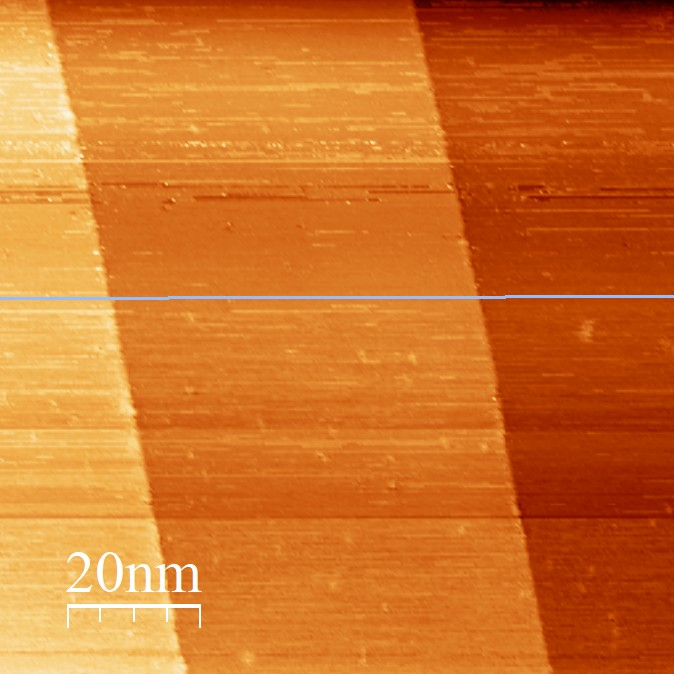
\includegraphics[width=0.58\linewidth]{../STM_data/Step/Step_final}
		\caption{Обзорный СТМ-кадр поверхности графита. Размер кадра $100\times100$~нм, ток 0.5~нА, напряжение 375~мВ.}
		\label{fig:2_step}
	\end{figure}
	
	\begin{figure}[H]
		\centering
		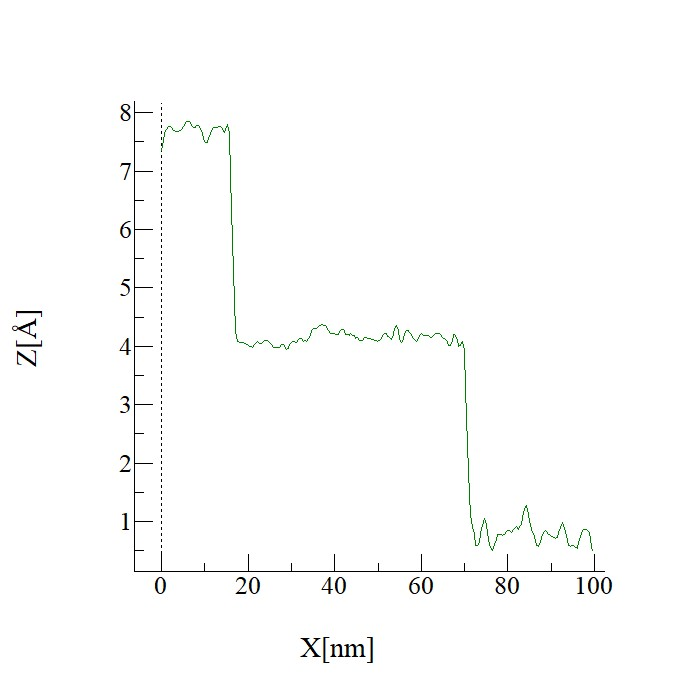
\includegraphics[width=0.6\linewidth]{../STM_data/Step/Step_final_Graph_enh.jpg}
		\caption{Профиль ступеньки графита, из которого видна высота ступеньки --- $3.5$~\AA.}
		\label{fig:2_step_anal}
	\end{figure}
	
	\subsection{Наблюдение атомной структуры}
	
	На рисунке \ref{fig:2_atomic} представлено полученное СТМ-изображение поверхности графита с атомной модуляцией. Мы видим отчетливую гексагональную структуру решетки, которая образуется двумя атомными слоями графита, смещенными друг относительно друга. Наблюдаемый нами гексагон --- точки с максимальной электронной плотностью, т.е. те места, где узлы двух слоев (синего и зеленого) совпадают (см. схему на рисунке \ref{fig:2_atomic}). Зная, что мы должны наблюдать правильный гексагон (экспериментально это можно было бы подтвердить, например, с помощью дифракции медленных электронов), мы можем по теореме косинусов определить реальное расстояние между атомами одного слоя, зная расстояние между соседними наблюдаемыми модуляциями. Межатомное расстояние, посчитанное таким образом, оказывается равным $1.4$~\AA. 
	
	\subsection{Зависимость СТМ-изображения атомной структуры от напряжения}
	
	На одном и том же участке было проведено несколько последовательных сканирований при различных напряжениях с целью найти зависимость профиля изображения от напряжения. Полученные кадры представлены на рисунке \ref{fig:2_different_volt}, а профили одного из рядов на каждом из них --- на рисунке \ref{fig:2_different_volt_profiles}. Из последнего видно, что с увеличением напряжения <<глубина>> профиля становится все меньше. Это наблюдение подтверждается в \cite{STM_Binnig}.
	
	\begin{figure}[H]
		\centering
		\includegraphics[width=0.6\linewidth]{Crystal_structure}
		\caption{Атомная структура поверхности графита, размер кадра $2.6\times2.6$~нм, ток $0.4$~нА, напряжение 25.6~мВ, расстояние между двумя модуляциями 2.33~\AA. На кадр нанесены две решетки слоев графита (синяя и зеленая), сдвинутых друг относительно друга, перекрытие которых дает наблюдаемую атомную модуляцию (красная).}
		\label{fig:2_atomic}
	\end{figure}
	
	\begin{figure}[H]
		\centering
		\includegraphics[width=0.5\linewidth]{../STM_data/STM_profiles/Graphs/Crystal_structure}
		\caption{Профиль изображения \ref{fig:2_atomic}, из которого получается расстояние между модуляциями 2.33~\AA. Измерено расстояние между несколькими модуляциями для накопления большей статистики.}
		\label{fig:2_atomic_g}
	\end{figure}
	
	\begin{figure}[H]
		\centering
		\subfigure[]{
			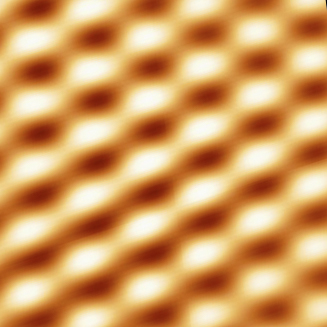
\includegraphics[width=0.36\linewidth]{../STM_data/STM_Profiles/Final_pictures/25}
		}	
		\subfigure[]{
			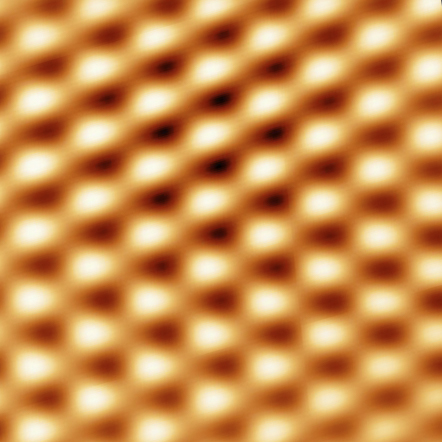
\includegraphics[width=0.36 \linewidth]{../STM_data/STM_Profiles/Final_pictures/64}
		}
		\subfigure[]{
			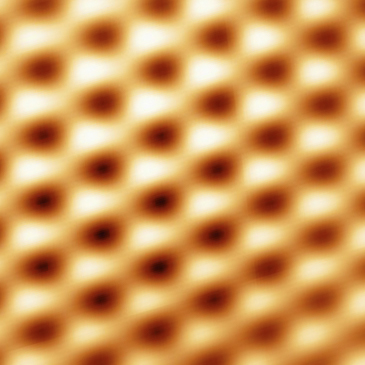
\includegraphics[width=0.36\linewidth]{../STM_data/STM_Profiles/Final_pictures/93}
		}	
		\subfigure[]{
			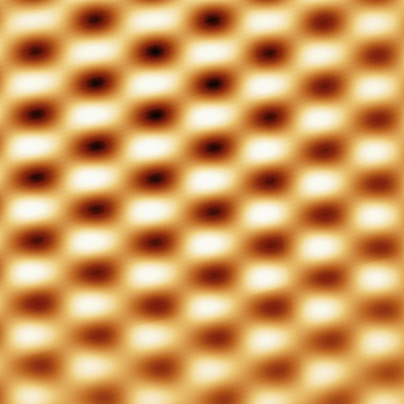
\includegraphics[width=0.36 \linewidth]{../STM_data/STM_Profiles/Final_pictures/150}
		}
		\subfigure[]{
			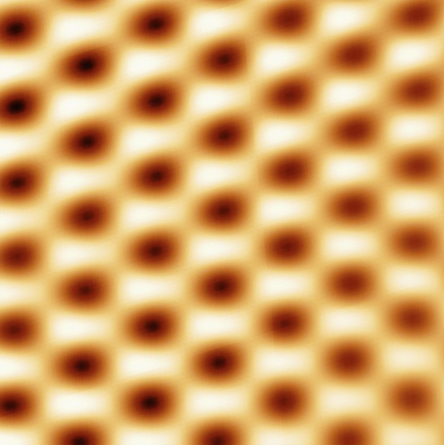
\includegraphics[width=0.36 \linewidth]{../STM_data/STM_Profiles/Final_pictures/200}
		}
		
		\caption{СТМ-изображение атомной структуры при различных напряжениях. Слева направо и сверху вниз при напряжении, соответственно: 25.6~мВ, 64.4~мВ, 93.3~мВ, 150.1~мВ, 200~мВ. Размеры всех изображений составляют $2.6\times2.6$~нм, ток --- 0.4~нА.}
		\label{fig:2_different_volt}
	\end{figure}

	\begin{figure}[H]
		\centering
		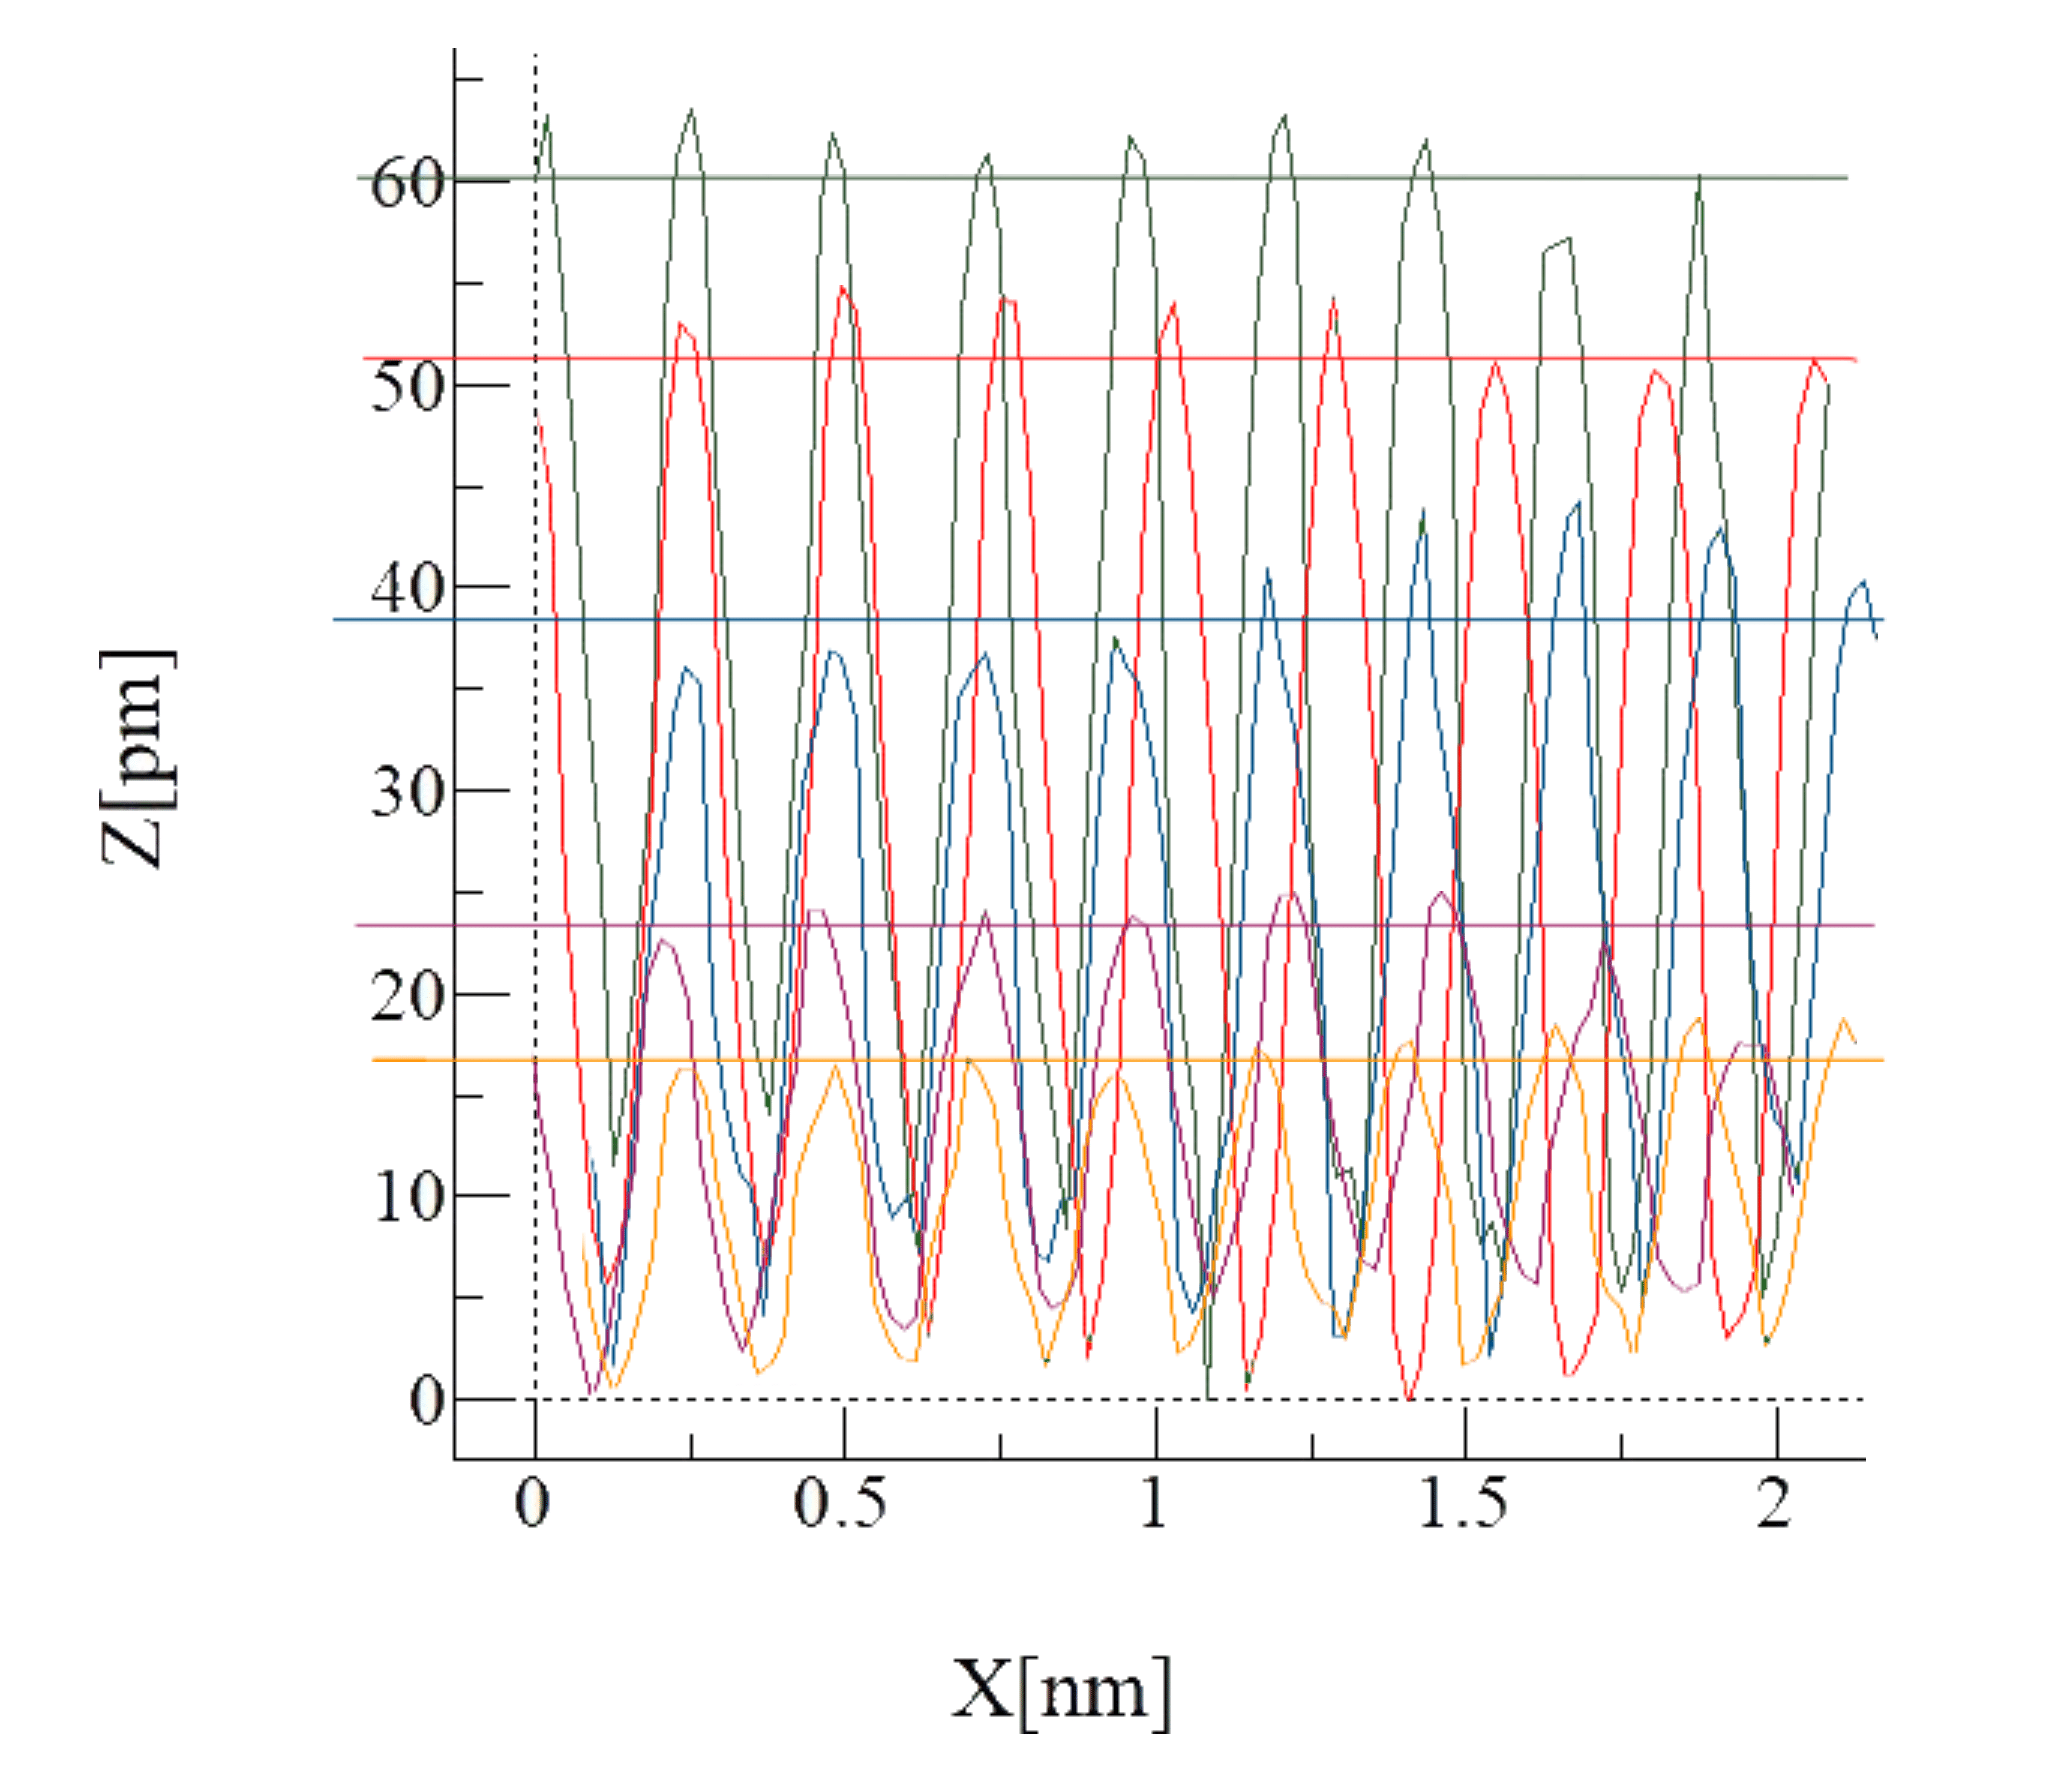
\includegraphics[width=0.9\linewidth]{../STM_data/STM_Profiles/Graphs/All_graphs}
		\caption{Профили атомного изображения при одинаковых токах (0.4~нА), но при различных напряжениях: зеленый --- 25.6~мВ, красный --- 64.4~мВ, синий --- 93.3~мВ, фиолетовый --- 150.1~мВ, оранжевый --- 200~мВ.}
		\label{fig:2_different_volt_profiles}
	\end{figure}


	
	\subsection{Наблюдение муара}
	
	В ходе выполнения сканирования было выявлено, что на поверхности графита присутствует муаровый узор. В связи с этим было принято решение провести дополнительное изучение этого эффекта.
	
	Увиденный нами муар представлен на рисунке \ref{fig:2_muar_image}. Наблюдаются атомные модуляции, а также модуляция сверхструктуры. Это подтверждает и Фурье-образ изображение (см. рисунок \ref{fig:2_muar_f}), на котором также видно две структуры: атомный гексагон (внутренний, маленький) и гексагон сверхструктуры (внешний, большой).
	
	В силу того, что графит имеет слоистую структуру, а в нашем образце отсутствуют примеси, которые могли бы вносить какие-то изменения в его структуру, единственным возможным способом появления муара является наличие двух повернутых относительно друг друга <<слоев>> графита (<<слои>> здесь подразумевают не один атомный слой, а объединение двух, см. пункт про атомную структуру). Чтобы подтвердить это предположение, мы решили смоделировать эти два повернутых <<слоя>>. Для этого было вычислено расстояние между двумя соседними элементами сверхструктуры (см. рисунок \ref{fig:2_muar_size}), которое оказалось равным $3.82$~нм. Реально было измерено расстояние не между двумя соседними элементами, а между элементами, находящимися через один, чтобы накопить большую статистику. Уже этого, зная устройство <<слоев>>, должно быть достаточно для построения модели. В качестве некоторой контрольной точки мы также измерили угол поворота решетки сверхструктуры относительно верхнего <<слоя>> из фурье-изображения \ref{fig:2_muar_f}, который оказался равен %ЧИСЛО
	
	После моделирования мы выяснили, что для достижения указанного периода сверхструктуры необходимо, чтобы <<слои>> были повернуты друг относительно друга на 6.2$^\circ$. При этом угол между верхним <<слоем>> графита и муром также оказался равен % ЧИСЛО
	Полученная нами модель представлена на рисунке \ref{fig:2_muar_model}.
	
	\begin{figure}[H]
		\centering
		\subfigure[]{
			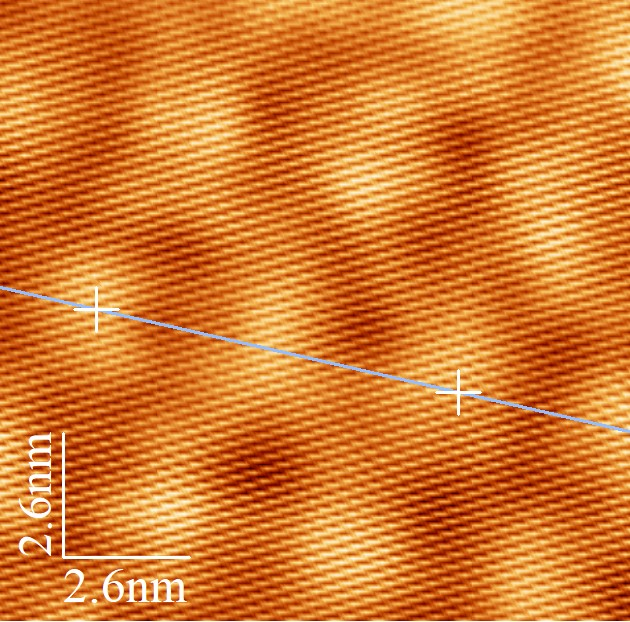
\includegraphics[width=0.45\linewidth]{../STM_data/Muar/Muar_final}
			\label{fig:2_muar_image}
		}
		\subfigure[]{
			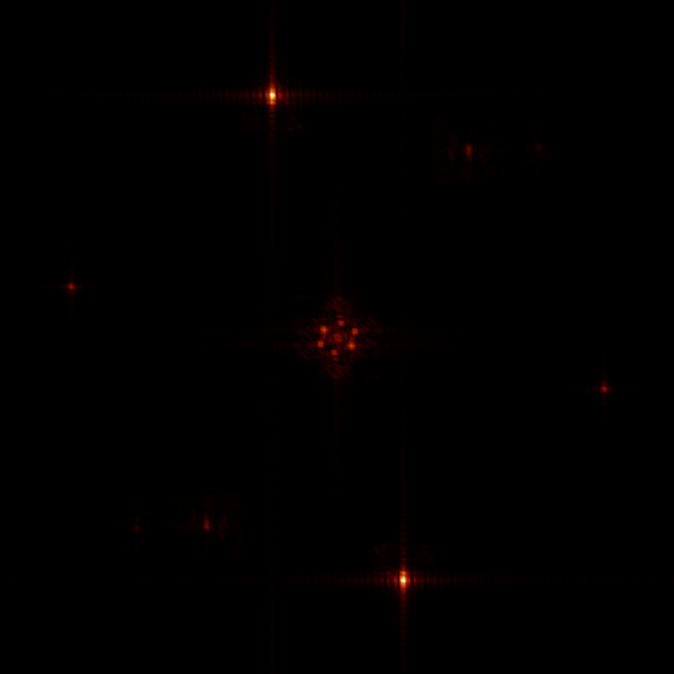
\includegraphics[width=0.45\linewidth]{../STM_data/Muar/Muar_final_f}
			\label{fig:2_muar_f}
		}
		\subfigure[]{
			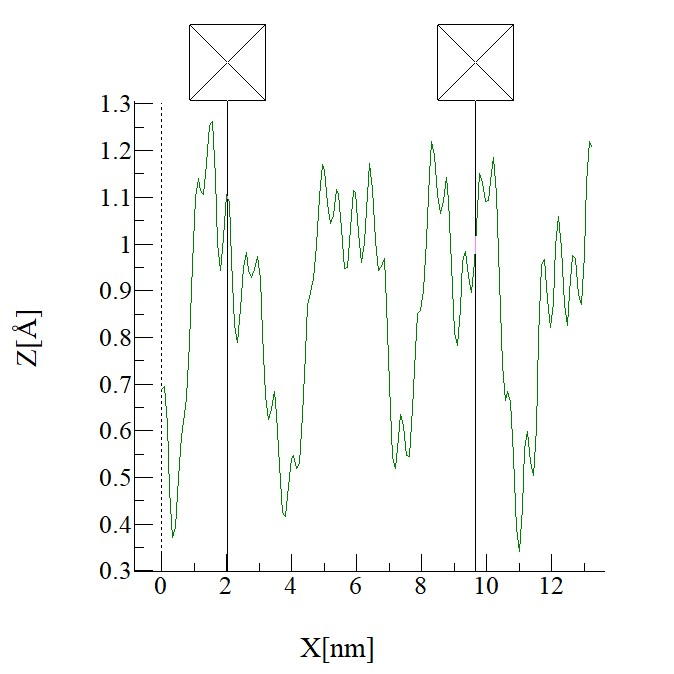
\includegraphics[width=0.6\linewidth]{../STM_data/Muar/Muar_final_g}
			\label{fig:2_muar_size}
		}
		\caption{СТМ-кадр графита с наблюдающимся муаром, размер изображения $13\times13$~нм, ток 0.3~нА, напряжение 297~мВ (a), его Фурье-образ (b), профиль для определения расстояния между элементами сверхструктуры, оказавшегося равным 3.82~нм (c).}
		\label{fig:2_muar}
	\end{figure}
	
	\begin{figure}[H]
		\centering
		
\includegraphics[width=0.9\linewidth]{../STM_data/Muar/Muar_model}
		\caption{Компьютерное моделирование сверхструктуры.}
		\label{fig:2_muar_model}
	\end{figure}
	
	\section{Выводы}
	
	В результате проведения лабораторной работы:
	
	\begin{enumerate}
		\item Расшифрован оже-спектр неизвестного образца. Из полученного спектра следует, что образец состоит из натрия, фтора, тулия и иттрия. Пики углерода и кислорода на оже-спектре происходят из остатков газа в вакуумной камере.
		
		\item Получен обзорный СТМ-кадр с моноатомной ступенькой. Измерена ее высота, которая оказалась равной 3.5~\AA, что согласуется с указанным в \cite{Article}.
		
		\item Получен СТМ-кадр атомной структуры, из которого получено межатомное расстояние в решетке графита: 1.4~\AA.
		
		\item Проведен эксперимент по поиску зависимости СТМ-изображения атомной структуры от напряжения, в ходе которого установлено, что с ростом напряжения <<глубина>> кадра уменьшается, что качественно подтверждается в \cite{STM_Binnig}.
		
		\item При сканировании обнаружен муар вызванный поворотом двух (или более) <<слоев>> решетки относительно друг друга. Было выяснено, что для получения такого рисунка муара <<слои>> должны быть повернуты друг относительно друга на $6.2^\circ$.
	\end{enumerate}
	
	\newpage
	
	\begin{thebibliography}{2}
		
		\bibitem{Auger} Handbook of Auger Electron Spectroscopy. /  Lawrence E. Davis, Noel C. MacDonald, Paul W. Palmberg, Greald E. Riach, Roland E. Wever --- Physical Electrinics Industries, Inc., February 1976.
		
		\bibitem{Auger_spectr} Описание работы оже-спектрометра. / ??
		
		\bibitem{STM} Общее описание СТМ GPI-300. / ??
		
		\bibitem{Article} Scanning tunneling microscopy and spectroscopy of the electronic local density of states of graphite surfaces near monoatomic step edges. / Y. Niimi, T. Matsui, H. Kambara, K. Tagami, M. Tsukada, and Hiroshi Fukuyama --- Tokyo, Japan : Department of Physics, University of Tokyo, February 24, 2006.
		
		\bibitem{Auge_diag} Анализ поверхности методами Оже- и рентгеновской фотоэлектронной спектроскопии. / Бриггса Д., Сиха М.М.
		
		\bibitem{Eltsov} Сверхвысоковакуумный сканирующий туннельный микроскоп GPI-300. / Ельцов К.Н. , А.Н. Климов, А.Н. Косяков, О.В. Объедков, В.Ю. Юров, В.М. Шевлюга --- Москва : Труды института общей физики им. А.М. Прохорова, 2003.
		
		\bibitem{STM_Binnig} Binnig, Gerd, and Heinrich Rohrer. ''Scanning tunneling microscopy.'' IBM Journal of research and development 44.1/2 (2000): 279.
		
	\end{thebibliography}
	
	
	\newpage
	
	% Оже-спектры выношу отдельно, по одному на страницу, чтобы не сидеть "а че там написано"
	
	
	
	
	
	
	

	

	
	
	
	
	
	
	
	
	
	
	
	
	
	
	
	
	
	
	
	
	
	
	
	
	
	
	
	
	
	
	
	
	
	
	
	
	
\end{document}